%%%%%%%%%%%%%%%%%%%%%%%%%%%%%%%%%%%%%%%%%%%%%%%%%%%%%%%%%%%%%%%%%%%%%%%%%%%%%%%%
\section{The Database}
%%%%%%%%%%%%%%%%%%%%%%%%%%%%%%%%%%%%%%%%%%%%%%%%%%%%%%%%%%%%%%%%%%%%%%%%%%%%%%%%
\begin{frame}
\frametitle{The Database}
\texttt{SQLite} is an open source database that has been around for a long time, is quite stable
\begin{itemize}
\item It’s a zero-configuration database
\item It doesn’t have a server. It is basically
a set of libraries that provide the database functionality
\item It’s a single-file database
\item It’s open source
\end{itemize}
\end{frame}
%------------------------------------------------------------------------------
\begin{frame}
\frametitle{\texttt{DbHelper}}
Android provides an elegant interface for your app to interact with an SQLite database
\begin{enumerate}
\item To access the database, you first need a helper class that provides a ``connection'' to
the database, creating the connection if it doesn’t already exist. This class, provided to
you by the Android framework, is called \alert{\texttt{SQLiteOpenHelper}}
\item The database class it returns is an instance of \alert{\texttt{SQLiteDatabase}}
\end{enumerate}

DbHelper offers (CRUD: create, read (query), update, and delete):
\begin{description}
\item [\texttt{insert()}] Inserts one or more rows into the database
\item [\texttt{query()}] Requests rows matching the criteria you specify
\item [\texttt{update()}] Replaces ones or more rows that match the criteria you specify
\item [\texttt{delete()}] Deletes rows matching the criteria you specify
\end{description}
\end{frame}
%------------------------------------------------------------------------------
\begin{frame}
\frametitle{\texttt{First Example}}
Create a new Java class in the same package as the rest of our
classes. Call this class \texttt{DBHelper}, and it will extend the \texttt{SQLiteOpenHelper} base
class from the framework. We then need to implement ;
\begin{itemize}
\item The class’s constructor
\item  \texttt{public abstract void onCreate (SQLiteDatabase db)}\\Called when the database is created for the first time. This is where the creation of tables and the initial population of the tables should happen
\item \texttt{public abstract void onUpgrade (SQLiteDatabase db, int oldVersion, int newVersion)}\\ Called when the database needs to be upgraded. The implementation should use this method to drop tables, add tables \dots
\end{itemize}

\end{frame}
%------------------------------------------------------------------------------
\begin{frame}[allowframebreaks,containsverbatim]
\frametitle{\texttt{DBHelper.java}}

\lstset{language=java, style=eclipse, breaklines=true, tabsize=2}
\begin{lstlisting}[caption=src/com/artemisa/yamba/DBHelper.java, basicstyle=\tiny,escapechar=$]
// .
// .
// .

public class DBHelper extends SQLiteOpenHelper { //  $\circled{1}$

	static final String TAG = DBHelper.class.getSimpleName();
	static final String DB_NAME = "timeline.db"; //  $\circled{2}$
	static final int DB_VERSION = 1; //
	static final String TABLE = "timeline";
	static final String C_ID = "id";
	static final String C_CREATED_AT = "created_at";
	static final String C_SOURCE = "source";
	static final String C_TEXT = "txt";
	static final String C_USER = "user";

	public DBHelper(Context context) { //  $\circled{3}$
		// TODO Auto-generated constructor stub

		super(context, DB_NAME, null, DB_VERSION);
	}

	// Called only once, first time the DB is created
	@Override
	public void onCreate(SQLiteDatabase db) { //  $\circled{4}$
		// TODO Auto-generated method stub
		String sql = "create table" + TABLE + " (" + C_ID
				+ " int primary key, " + C_CREATED_AT + " int, " + C_SOURCE + " text, " + C_USER
				+ " text, " + C_TEXT + " text)";
		db.execSQL(sql);
		Log.d(TAG, "onCreated sql:" + sql);
	}

	// Called whenever newVersion != to oldVersion
	@Override
	public void onUpgrade(SQLiteDatabase db, int oldVersion, int newVersion) { //  $\circled{5}$
		// TODO Auto-generated method stub
		// Typically do ALTER TABLE statements, but...we're just in development,
		// so:
		db.execSQL("drop table if exists " + TABLE); // drops the old database
		Log.d(TAG, "onUpdated");
		onCreate(db); // run onCreate to get new database
	}

}

\end{lstlisting}
\end{frame}
%------------------------------------------------------------------------------
%------------------------------------------------------------------------------
\begin{frame}[allowframebreaks,containsverbatim]
\frametitle{\texttt{Update UpdaterService}}

\lstset{language=java, style=eclipse, breaklines=true, tabsize=2}
\begin{lstlisting}[caption=src/com/artemisa/yamba/UpdaterService.java, basicstyle=\tiny,escapechar= $]
// .
// .
// .

public class UpdaterService extends Service {
	private static final String TAG = "UpdaterService";
	private static final int DELAY = 60000; // a minute
	private boolean runFlag = false;
	private Updater updater;
	private YambaApplication yamba; // $\circled{1}$
	private DBHelper dbHelper; // $\circled{2}$

	@Override
	public IBinder onBind(Intent arg0) {
		// TODO Auto-generated method stub
		return null;
	}

	@Override
	public void onCreate() {
		// TODO Auto-generated method stub
		super.onCreate();
		yamba = (YambaApplication) getApplication(); $\circled{3}$
		dbHelper = new DBHelper(yamba); $\circled{4}$
		updater = new Updater();

		Log.d(TAG, "onCreated");

	}

	// .
	// .
	// .

	/*
	 * Threads tha permos the actual update from the online service
	 */
	private class Updater extends Thread {
		List<Twitter.Status> timeline;

		private Updater() {
			super("UpdaterService-Updater");
			// TODO Auto-generated constructor stub
		}

		@Override
		public void run() {
			UpdaterService updaterService = UpdaterService.this;
			while (updaterService.runFlag) {
				Log.d(TAG, "Updater running");
				try {
					try {
						// Get the timeline from the cloud
						timeline = updaterService.yamba.getTwitter() 
								.getFriendsTimeline(); // $\circled{4}$  
					} catch (TwitterException e) {
						Log.e(TAG, "Failed to connect to twitter service", e);
					}

					// Open the database for writing
					SQLiteDatabase db = dbHelper.getWritableDatabase(); // $\circled{5}$

					// Loop over the timeline and print it out
					ContentValues values = new ContentValues(); // $\circled{6}$
					for (Twitter.Status status : timeline) { // $\circled{7}$
						// Insert into database
						values.clear(); // $\circled{8}$
						values.put(DBHelper.C_ID, status.id);
						values.put(DBHelper.C_CREATED_AT,
								status.createdAt.getTime());
						values.put(DBHelper.C_SOURCE, status.source);
						values.put(DBHelper.C_TEXT, status.text);
						values.put(DBHelper.C_USER, status.user.name);
						try {
							db.insertOrThrow(DBHelper.TABLE, null, values); // $\circled{9}$
							Log.d(TAG, String.format("%s: %s",
									status.user.name, status.text));
						} catch (SQLException e) {
							// TODO Auto-generated catch block
							Log.e(TAG, e.toString());
							e.printStackTrace();
						}

					}
					db.close(); // $\circled{10}$

					Log.d(TAG, "Updater ran");
					Thread.sleep(DELAY);
				} catch (InterruptedException e) {
					updaterService.runFlag = false;
				}
			}
		}

	}

}

\end{lstlisting}
\end{frame}
%------------------------------------------------------------------------------
\begin{frame}
\frametitle{Testing the service}
To see whether your database schema was created properly:
\begin{itemize}
\item Open up your terminal or command-line window
\item Type \texttt{adb shell} to connect to your running emulator or physical phone
\item Change the directory to the location of your database file by typing \texttt{cd /data/data/com.artemisa.yamba/databases/}
\item Connect to the database with the \texttt{sqlite3 timeline.db} command. At this point, you can send commands to your SQLite database:
\begin{itemize}
\item \texttt{sqlite> .schema;}
\item \texttt{sqlite> SELECT * FROM timeline;}
\end{itemize}
\end{itemize}

\end{frame}
%------------------------------------------------------------------------------
\begin{frame}[fragile]
\frametitle{Git}
\begin{enumerate}
\item \texttt{git status}
\item \texttt{git add .}
\item \texttt{git status}
\item \texttt{git commit -a -m ``Database''}
\end{enumerate}

\end{frame}
%------------------------------------------------------------------------------
\begin{frame}[fragile]
\frametitle{Refactoring Status Data}
The work we did previously for the \texttt{UpdaterService} is not ideal for supporting our next
user of this data: the \texttt{TimelineActivity}. Since \texttt{TimelineActivity} will also need to access
the same database and fetch the same data, it would be better if we would share some
of the same functionality between the \texttt{UpdaterService} and the \texttt{TimelineActivity}.
In order to do that, we’ll create a new Java class, \texttt{StatusData}, and make it the common
container for database-related functionality . It will be hiding (encapsulating)
SQLite in a higher-level class accessible to other parts of the Yamba application.
The rest of our app will then just ask for \texttt{StatusData}
\end{frame}
%------------------------------------------------------------------------------
\begin{frame}[allowframebreaks,containsverbatim]
\frametitle{\texttt{StatusData.java}}
\lstset{language=java, style=eclipse, breaklines=true, tabsize=2}
\begin{lstlisting}[caption=src/com/artemisa/yamba/StatusData.java, basicstyle=\tiny,escapechar= $]
// .
// .
// .
public class StatusData {
	static final String TAG = StatusData.class.getSimpleName();
	static final String DB_NAME = "timeline.db";
	static final int DB_VERSION = 1; //
	static final String TABLE = "timeline";
	static final String C_ID = "id";
	static final String C_CREATED_AT = "created_at";
	static final String C_SOURCE = "source";
	static final String C_TEXT = "txt";
	static final String C_USER = "user";

	private static final String[] MAX_CREATED_AT_COLUMNS = { "max("
			+ StatusData.C_CREATED_AT + ")" }; // $\circled{1}$

	public class DBHelper extends SQLiteOpenHelper { // $\circled{2}$

		public DBHelper(Context context) {
			// TODO Auto-generated constructor stub

			super(context, DB_NAME, null, DB_VERSION);
		}

		// Called only once, first time the DB is created
		@Override
		public void onCreate(SQLiteDatabase db) {
			// TODO Auto-generated method stub
			String sql = "create table " + TABLE + " (" + C_ID
					+ " int primary key, " + C_CREATED_AT + " int, " + C_SOURCE
					+ " text, " + C_USER + " text, " + C_TEXT + " text)";
			db.execSQL(sql);
			Log.d(TAG, "onCreated sql:" + sql);
		}

		// Called whenever newVersion != to oldVersion
		@Override
		public void onUpgrade(SQLiteDatabase db, int oldVersion, int newVersion) {
			// TODO Auto-generated method stub
			// Typically do ALTER TABLE statements, but...we're just in
			// development,
			// so:
			db.execSQL("drop table if exists " + TABLE); // drops the old database
			Log.d(TAG, "onUpdated");
			onCreate(db); // run onCreate to get new database
		}
	}

	private DBHelper dbHelper; // $\circled{3}$

	public StatusData(Context context) { // $\circled{4}$
		dbHelper = new DBHelper(context);
		Log.i(TAG, "Initialized data");
	}

	public void close() {
		dbHelper.close();
	}

	public void insertOrIgnore(ContentValues values) { // $\circled{5}$
		Log.d(TAG, "insertOrIgnore" + values);
		// Open the database for writing
		SQLiteDatabase db = dbHelper.getWritableDatabase();

		try {
			db.insertWithOnConflict(StatusData.TABLE, null, values,
					SQLiteDatabase.CONFLICT_IGNORE);
		} finally {
			db.close();
		}
	}

	/**
	 * 
	 * @return Timestamp of the latest status we ahve it the database
	 */
	public long getLatestStatusCreatedAtTime() { // $\circled{6}$
		SQLiteDatabase db = this.dbHelper.getReadableDatabase();
		try {
			Cursor cursor = db.query(TABLE, MAX_CREATED_AT_COLUMNS, null, null,
					null, null, null);
			try {
				return cursor.moveToNext() ? cursor.getLong(0) : Long.MIN_VALUE;
			} finally {
				cursor.close();
			}
		} finally {
			db.close();
		}
	}

}

\end{lstlisting}
\end{frame}
%------------------------------------------------------------------------------
%------------------------------------------------------------------------------
\begin{frame}[allowframebreaks,containsverbatim]
\frametitle{\texttt{YambaApplication.java}}

\lstset{language=java, style=eclipse, breaklines=true, tabsize=2}
\begin{lstlisting}[caption=src/com/artemisa/yamba/YambaApplication.java, basicstyle=\tiny,escapechar= $]
// .
// .
// .
public class YambaApplication extends Application implements
		OnSharedPreferenceChangeListener {
	private static final String TAG = YambaApplication.class.getSimpleName();
	private Twitter twitter;
	private SharedPreferences prefs;

	private StatusData statusData; // $\circled{1}$

	public StatusData getStatusData() { // $\circled{2}$
		return statusData;
	}

	@Override
	public void onCreate() {
		// TODO Auto-generated method stub
		super.onCreate();

		prefs = PreferenceManager.getDefaultSharedPreferences(this);
		prefs.registerOnSharedPreferenceChangeListener(this);

		statusData = new StatusData(this); // $\circled{3}$
		Log.i(TAG, "onCreated");
	}

	// Connects to the online service and puts the latest statuses into DB.
	// Returns the count of new statuses
	public synchronized int fetchStatusUpdates() { // $\circled{4}$
		Log.d(TAG, "Fetching status updates");
		try {
			List<Status> statusUpdates = getTwitter().getFriendsTimeline();
			long latestStatusCreatedAtTime = this.getStatusData()
					.getLatestStatusCreatedAtTime();
			int count = 0;
			ContentValues values = new ContentValues();
			for (Status status : statusUpdates) {
				values.put(StatusData.C_ID, status.getId());
				long createdAt = status.getCreatedAt().getTime();
				values.put(StatusData.C_CREATED_AT, createdAt);
				values.put(StatusData.C_TEXT, status.getText());
				values.put(StatusData.C_USER, status.getUser().getName());
				Log.d(TAG, "Got update with id " + status.getId() + ". Saving");
				this.getStatusData().insertOrIgnore(values);
				if (latestStatusCreatedAtTime < createdAt) {
					count++;
				}
			}
			Log.d(TAG, count > 0 ? "Got " + count + " status updates"
					: "No new status updates");
			return count;
		} catch (RuntimeException e) {
			Log.e(TAG, "Failed to fetch status updates", e);
			return 0;
		}
	}


	// .
	// .
	// .

}

\end{lstlisting}
\end{frame}
%------------------------------------------------------------------------------
%------------------------------------------------------------------------------
\begin{frame}[allowframebreaks,containsverbatim]
\frametitle{\texttt{UpdaterService.java}}

\lstset{language=java, style=eclipse, breaklines=true, tabsize=2}
\begin{lstlisting}[caption=src/com/artemisa/yamba/UpdaterService.java, basicstyle=\tiny,escapechar= $]
// .
// .
// .
public class UpdaterService extends Service {
	// .
	// .
	// .

	/*
	 * Threads tha permos the actual update from the online service
	 */
	private class Updater extends Thread { 

		private Updater() {
			super("UpdaterService-Updater");
			// TODO Auto-generated constructor stub
		}

		@Override
		public void run() {
			UpdaterService updaterService = UpdaterService.this;
			while (updaterService.runFlag) {
				Log.d(TAG, "Updater running");
				try {
					try {
						// Get the timeline from the cloud
						YambaApplication yamba = (YambaApplication) updaterService.getApplication(); // $\circle{1}$
						int newUpdates = yamba.fetchStatusUpdates(); // $\circle{2}$
						if (newUpdates>0){ // $\circle{1}$
							Log.d(TAG, "We have a new status");
						}
						Thread.sleep(DELAY);
					} catch (TwitterException e) {
						Log.e(TAG, "Failed to connect to twitter service", e);
					}

					
				} catch (InterruptedException e) {
					updaterService.runFlag = false;
				}
			}
		}

	}

}


\end{lstlisting}
\end{frame}
%------------------------------------------------------------------------------
\begin{frame}[containsverbatim]
\frametitle{Summary}

\begin{center}
\includegraphics[width= 0.40 \textwidth]{database.eps}
\end{center}



\end{frame}
%------------------------------------------------------------------------------

\begin{frame}[fragile]
\frametitle{Git}
\begin{enumerate}
\item \texttt{git status}
\item \texttt{git add .}
\item \texttt{git status}
\item \texttt{git commit -a -m ``Database with StatusData''}
\item \texttt{git push -u carmelocuenca master}
\end{enumerate}

\end{frame}
%------------------------------------------------------------------------------